\chapter{Analytical Model and Preliminary Results}
In this chapter first a framework for the analysis that is performed is presented, later the basic model that is used for the analysis is presented and later calibrated and verified with experimental data available in the literature. Finally preliminary results are presented that will define the general view for the proposed research

\section{Analytical Model}

\subsection{Cantilever Column}
This study focuses on the behavior of a Single Degree of Freedom System representing a Cantilever Reinforced Concrete Column. The column is modeled as shown in \fref{fig:Structural_Model} This structure is modeled in OpenSeesPy \cite{McKenna2010}\cite{Zhu2018} using the $forceBeamColumn$ element \cite{Scott}. The forceBeamColumn element is used with two-point Gauss-Radau integration applied in the hinge regions and two-point Gauss integration applied on the element interior for a total of six integration points \cite{Scott}. The force based formulation requires only a single element to accurately represent the full nonlinear deformation of the member and the integration scheme selected prevents the loss of objectivity during softening response while also providing integration points at the member ends \cite{Calabrese2010},\cite{Scott}. The element requires the length of plasticity be defined at each end of the member, for which the tension based rectangular plastic hinge length is calculated using the following expressions \cite{Goodnight2013}:

\begin{equation}
    L_{pc}=k*L_{eff} + 0.4D
    \label{eq:LP_Comp}
\end{equation}
\begin{equation}
	k=0.2*(Fu/Fy - 1) \leqslant 0.08
	\label{eq:K_Lp}
\end{equation}
\begin{equation}
    L_{pt}=L_{pc}+\gamma*D
    \label{eq:LP_Tension}
\end{equation}

For Single Bending
\begin{equation}
    \gamma=0.33
    \label{eq:Gamma_LPt}
\end{equation}

The two-point Gauss-Radau integration is applied such that each end node integration is weighted equal to the specified plastic hinge length, as illustrated in \fref{fig:Fiber_PlasticHinge}. Therefore, strains recorded at the end sections represent accurate values even in the case where deformation localizes to the ends from strain softening behavior. For the case of the cantilever column considered, only one plastic hinge length is defined, and the opposite end is given an arbitrary unit length. 

\begin{figure}[htbp]
	\centering
	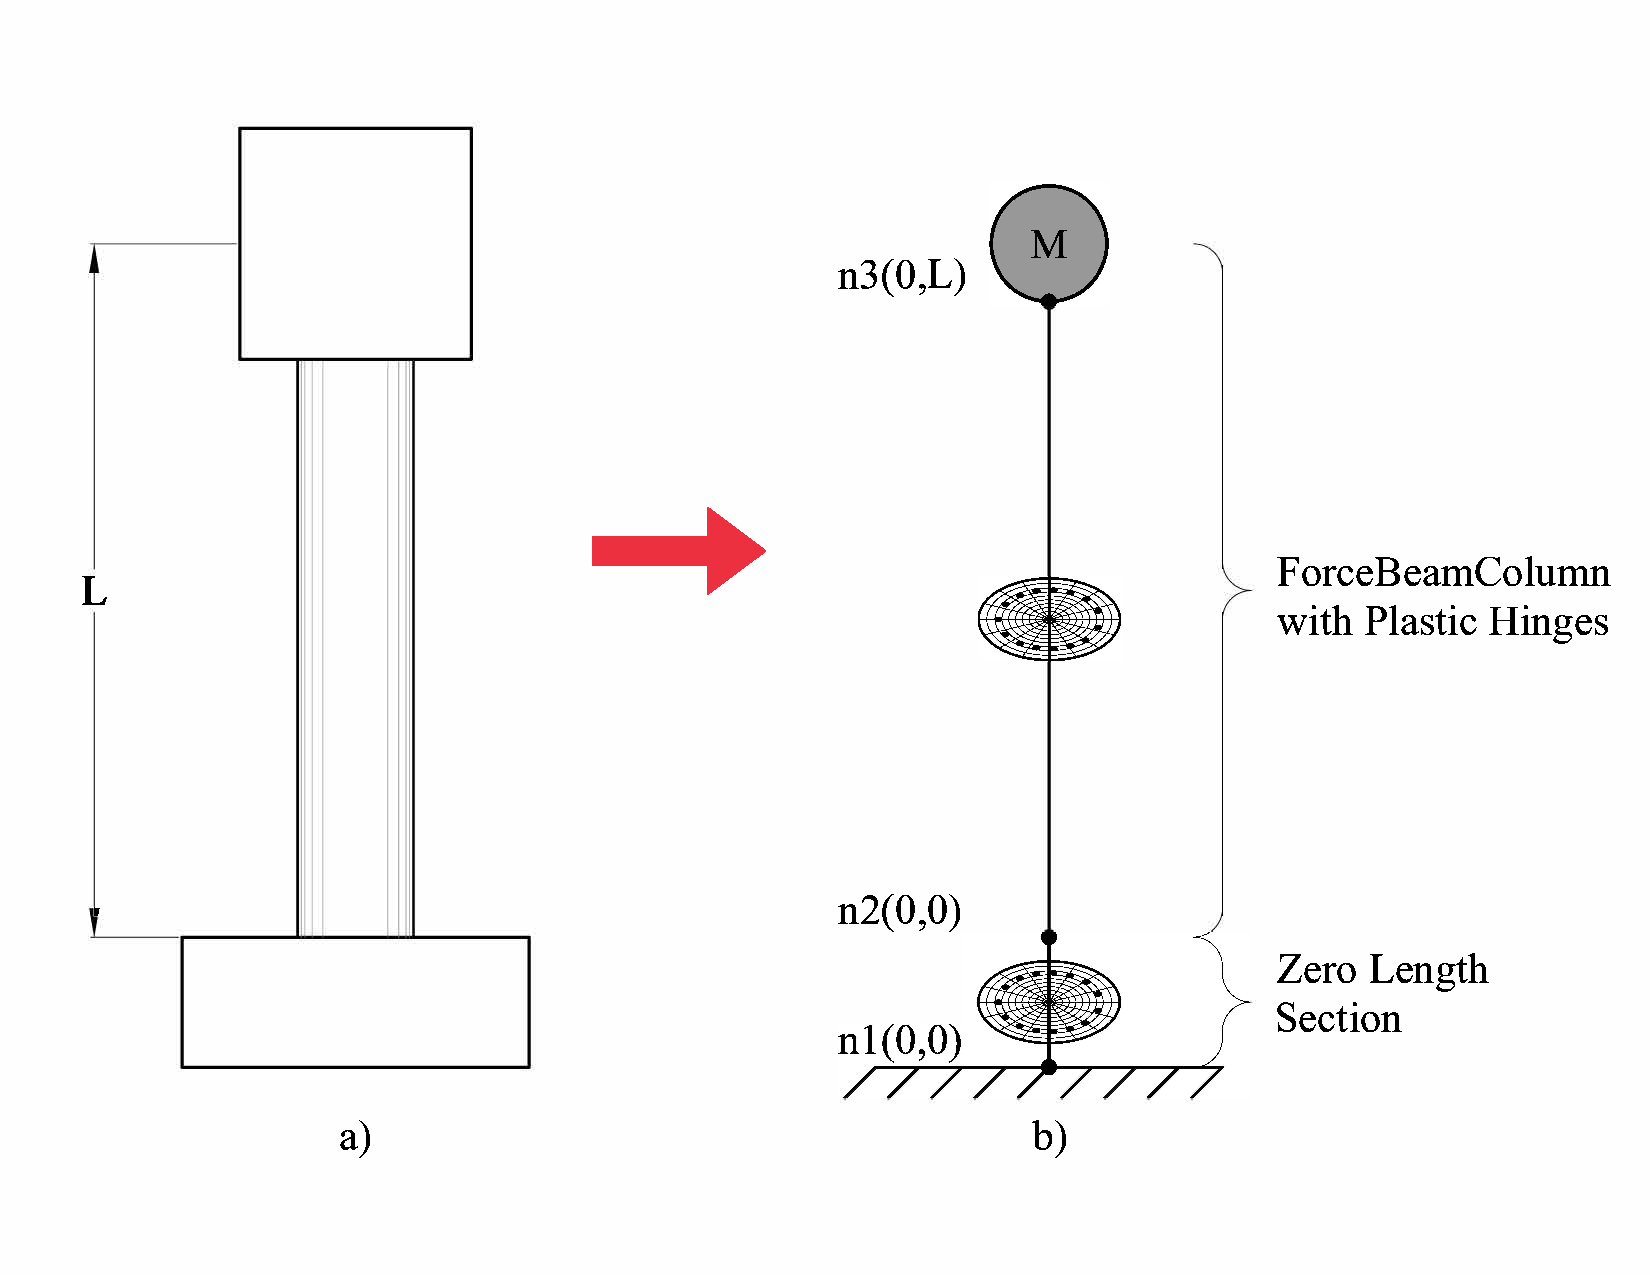
\includegraphics[width=1.0\textwidth]{Chapter-5/figs/StructuralModel_01}
	\caption{Structural Model a) SDOF Column b) Structural Model}
	\label{fig:Structural_Model}
\end{figure}

\begin{figure}[htbp]
	\centering
	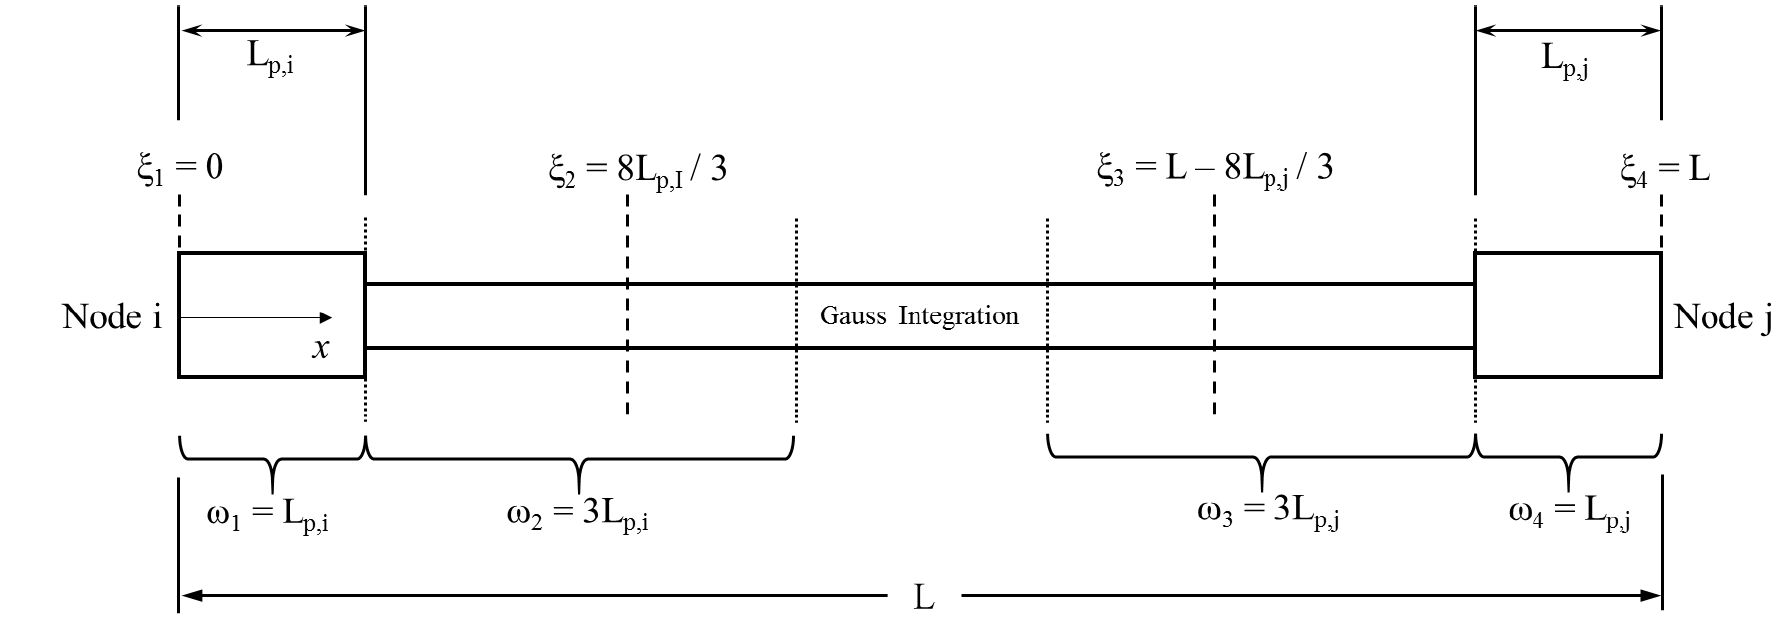
\includegraphics[width=0.9\textwidth]{Chapter-5/figs/fbc_PlasticHinge}
	\caption{End point plastic hinge method \cite{Scott}}
	\label{fig:Fiber_PlasticHinge}
\end{figure}

The section of the column is shown in \fref{fig:ColumnSection}, the section is discretized with concrete and steel material fibers. Concrete fibers are modeled using the $Concrete01$ material, modified for confined material strength based on the Mander confined concrete model \cite{Mander1988}. The $Steel02$ material, based on the Giuffre-Menegotto-Pinto model \cite{Filippou1983} and it is used for the longitudinal reinforcement with recommended parameters ($b = 0.01, R0 = 20, cR1 = 0.925, cR2 = 0.15$). 

\begin{figure}[htbp]
	\centering
	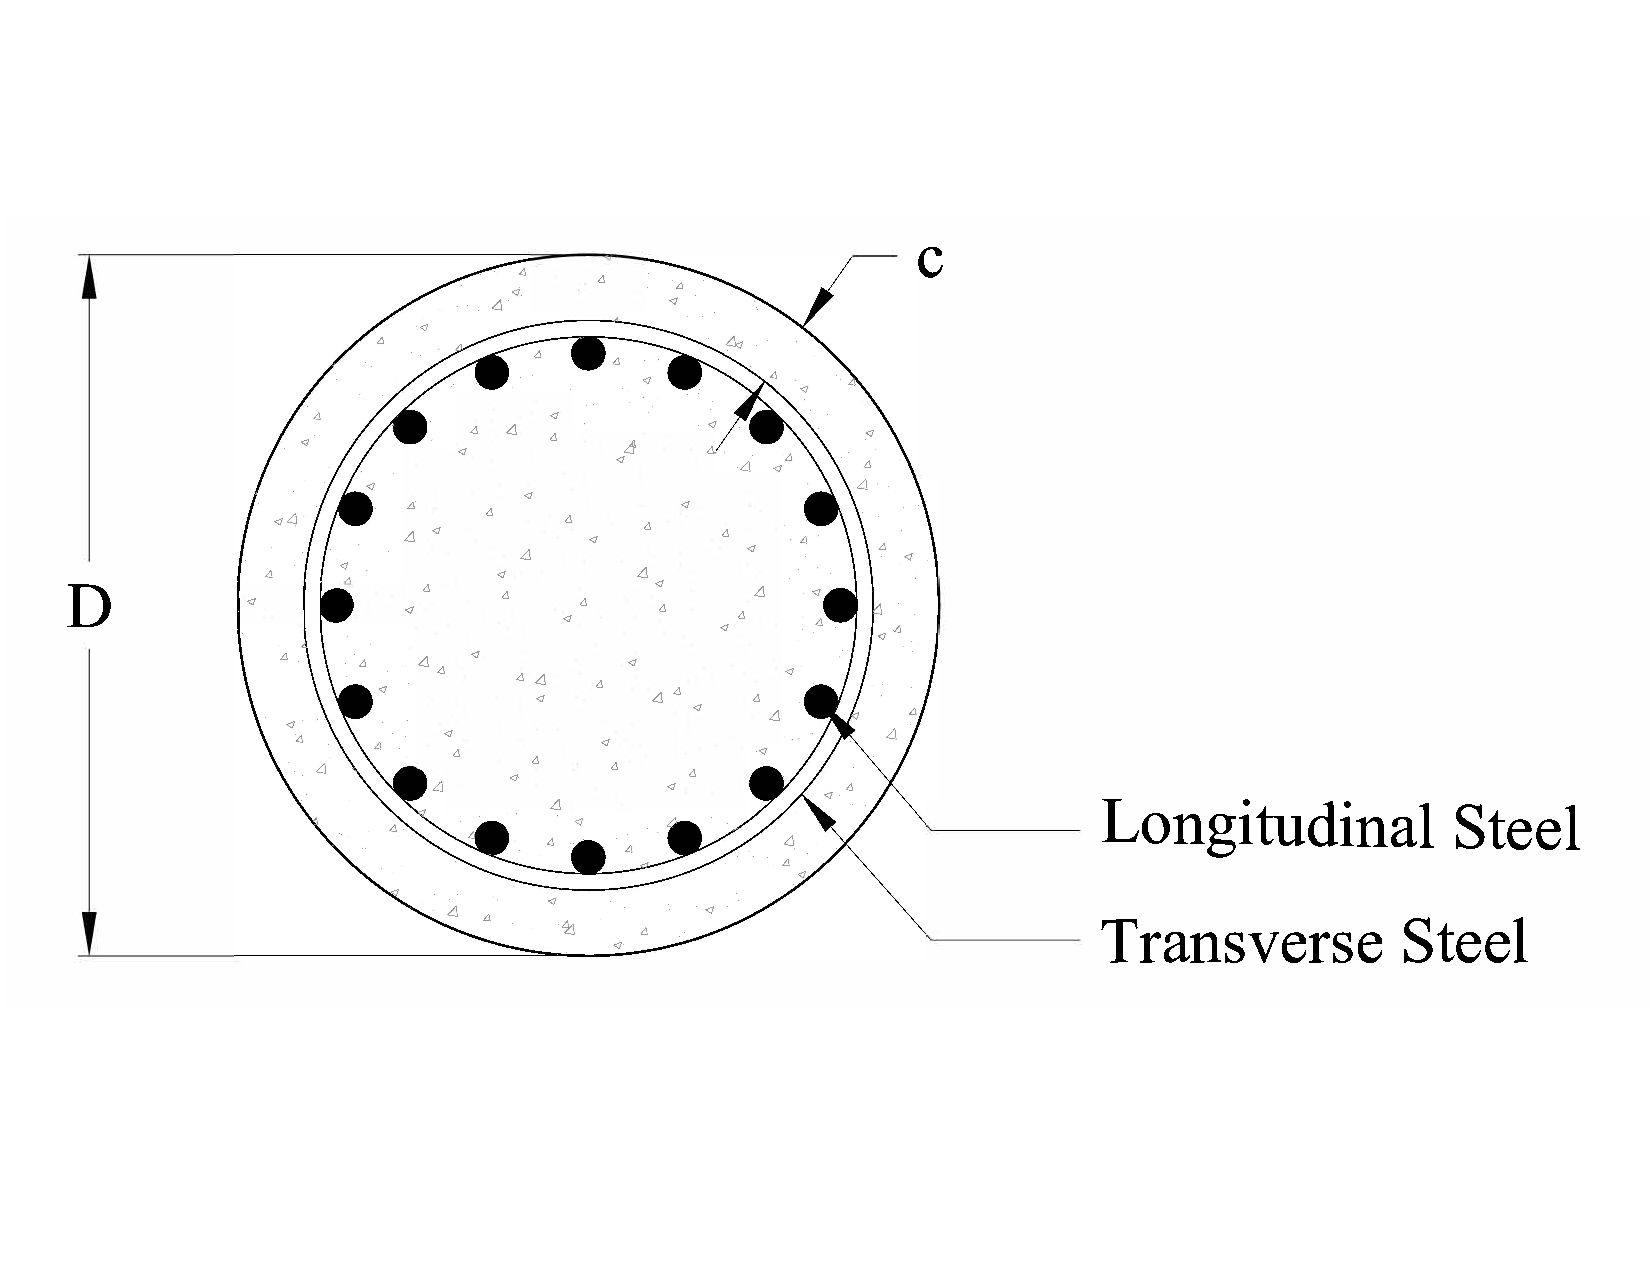
\includegraphics[width=0.7\textwidth]{Chapter-5/figs/StructuralModel_Section}
	\caption{Section of the RC Column}
	\label{fig:ColumnSection}
\end{figure}

\subsection{Strain Penetration Component}

The strain penetration is necessary to be considered to take into account the additional deformation due to anchorage of the reinforcement into the foundation, since the strains of tension in the reinforcement will drop to zero at a depth equal to the true development length of the rebar \cite{Priestley2007}. Experimental studies have generally reported that this end rotation contributes up to 35\% to the lateral deformation of flexural members\cite{Zhao2007} and it is therefore important to incorporate into the analytical model. A way to capture this effect is by using a zero-length section element implemented in nonlinear fiber-based analysis of concrete structures, this is available in the material library of OpenSeesPy as $Bond SP1$ \cite{Zhao2007} this is material model used for the steel fibers of the zero-length section element. 

The required parameters for this model are:
\begin{itemize}
	\item $F_{y}$ Yield strength of the reinforcement steel
	\item $S_{y}$ Rebar slip at member interface under yield stress (see \eref{eq.Rebar_Slip})
	\item $F_{u}$ Ultimate strength of the reinforcement steel
	\item $S_{u}$ Rebar slip at the loaded end at the bar fracture strength a value of $35 S_{y}$ is recommended \cite{Zhao2007}
	\item $b$ Initial hardening ratio in the monotonic slip vs. bar stress response $b=0.45$ is recommended \cite{Zhao2007}
	\item $R$ Pinching factor for the cyclic slip vs. bar response $R=1.01$ is recommended \cite{Zhao2007}
	\item $d_b$ Rebar diameter
	\item $f'c$ Concrete compressive strength of the adjoining connection member
	\item $\alpha$ Parameter used in the local bond-slip relation and can be taken as $\alpha=0.4$ in accordance with CEB-FIP Model Code 90 \cite{CEB1993}
\end{itemize}

Bar slip is calculated as:
\begin{equation}
	S_{y}(in)=0.1\left(\frac{d_{b}F_{y}}{4000\sqrt{f'_{c}}}\left(2\alpha+1\right)\right)^{\frac{1}{\alpha}}+0.013 (in)
	\label{eq.Rebar_Slip}
\end{equation}
\subsection{Design Limit States}
Design limit states are defined on the basis of strains in the material since they can more accurately represent the different performance level of a structure. Structure limit states are defined for tension strains in the rebars or compression strains in the concrete core. The values recommended in typical performance based design of reinforced concrete bridge columns are shown in Table  \ref{tab:DesignLimitStates}. The serviceability limit states correspond to the compression strain at which concrete cover begins to crush and the peak tension strain which results in residual crack widths of approximately 1 mm. These limits are generally accepted as nominal limit states for RC members. The compression limit state for damage control is defined by the expresion shown in Eq. \ref{eq:ec_DamageControl} and it refers to the compression strain in the confined concrete at which fracture of the transverse reinforcement confining the core occurs \cite{Priestley2007}. This equation is obtained using the strain-energy balance between that absorbed by the confined core concrete and the capacity of the confining steel. The tension damage control limit state is defined by the strain at the onset of buckling which can be expressed according to \ref{eq:es_DamageControl}, this equation demonstrated accurate predictions of the onset of bar buckling on physical tests in SDOF Concrete Column \cite{Goodnight2016}.

\begin{equation}
    \varepsilon_{c,spiral yield}=0.009-0.3\frac{A_{st}}{A_{g}} +3.9\frac{f_{yhe}}{E_{s}}
    \label{eq:ec_DamageControl}
\end{equation}

\begin{equation}
    \varepsilon_{s,BB}=0.03+700\rho_{s}  \frac{f_{yhe}}{E_{s}} -0.1\frac{P}{f'_{c}A_{g}}
    \label{eq:es_DamageControl}
\end{equation}


\begin{table}[htbp]
	\caption{Design Limit States}
	\label{tab:DesignLimitStates}
	\centering	
		\begin{tabular}{|l|c|c|}
		\hline
		\cellcolor[HTML]{CC0000}{\color[HTML]{FFFFFF}Limit State} & \cellcolor[HTML]{CC0000}{\color[HTML]{FFFFFF}Concrete Limit State $\varepsilon_{c} (in/in)$} & \cellcolor[HTML]{CC0000}{\color[HTML]{FFFFFF}Reinforcing Steel Limit State $\varepsilon_{s} (in/in)$}\\  \hline	
		Serviciability       & 0.004                           & 0.015  \\  \hline	
		Damage Control       & Eq. \ref{eq:ec_DamageControl}   & Eq. \ref{eq:es_DamageControl}\\  \hline
		\end{tabular}
\end{table}
 
\section{Comparison with existing physical Tests}
\subsection{Pristine Condition Columns}

One of the tests performed at NC State by Goodnight et al \citep{Goodnight2013} is used to calibrate the parameters used in the analytical model. The 

\subsection{Accelerated Corrosion Columns}
\lipsum[3]

\section{Analytical Framework}

An overall analytical framework is established such that several analysis can be performed. From this analysis it is possible to determine the effects of damage in the performance of structures. The proposed analytical framework consists in:

\begin{enumerate}
	\item Geometrical Properties of the SDOF column 
	\item Properties of the material are evaluated (i.e. water to cement ratio, cover)
	\item For equal periods of time the Time Dependent Properties are modified
	\item Nonlinear Time History Analysis are performed for discrete events or sequence of events
	\item Results are obtained and evaluated
\end{enumerate}

This procedure has been summarized in the form of a flow chart presented in \fref{fig:NLTHA_Framework}

\begin{figure}[htbp]
	\centering
	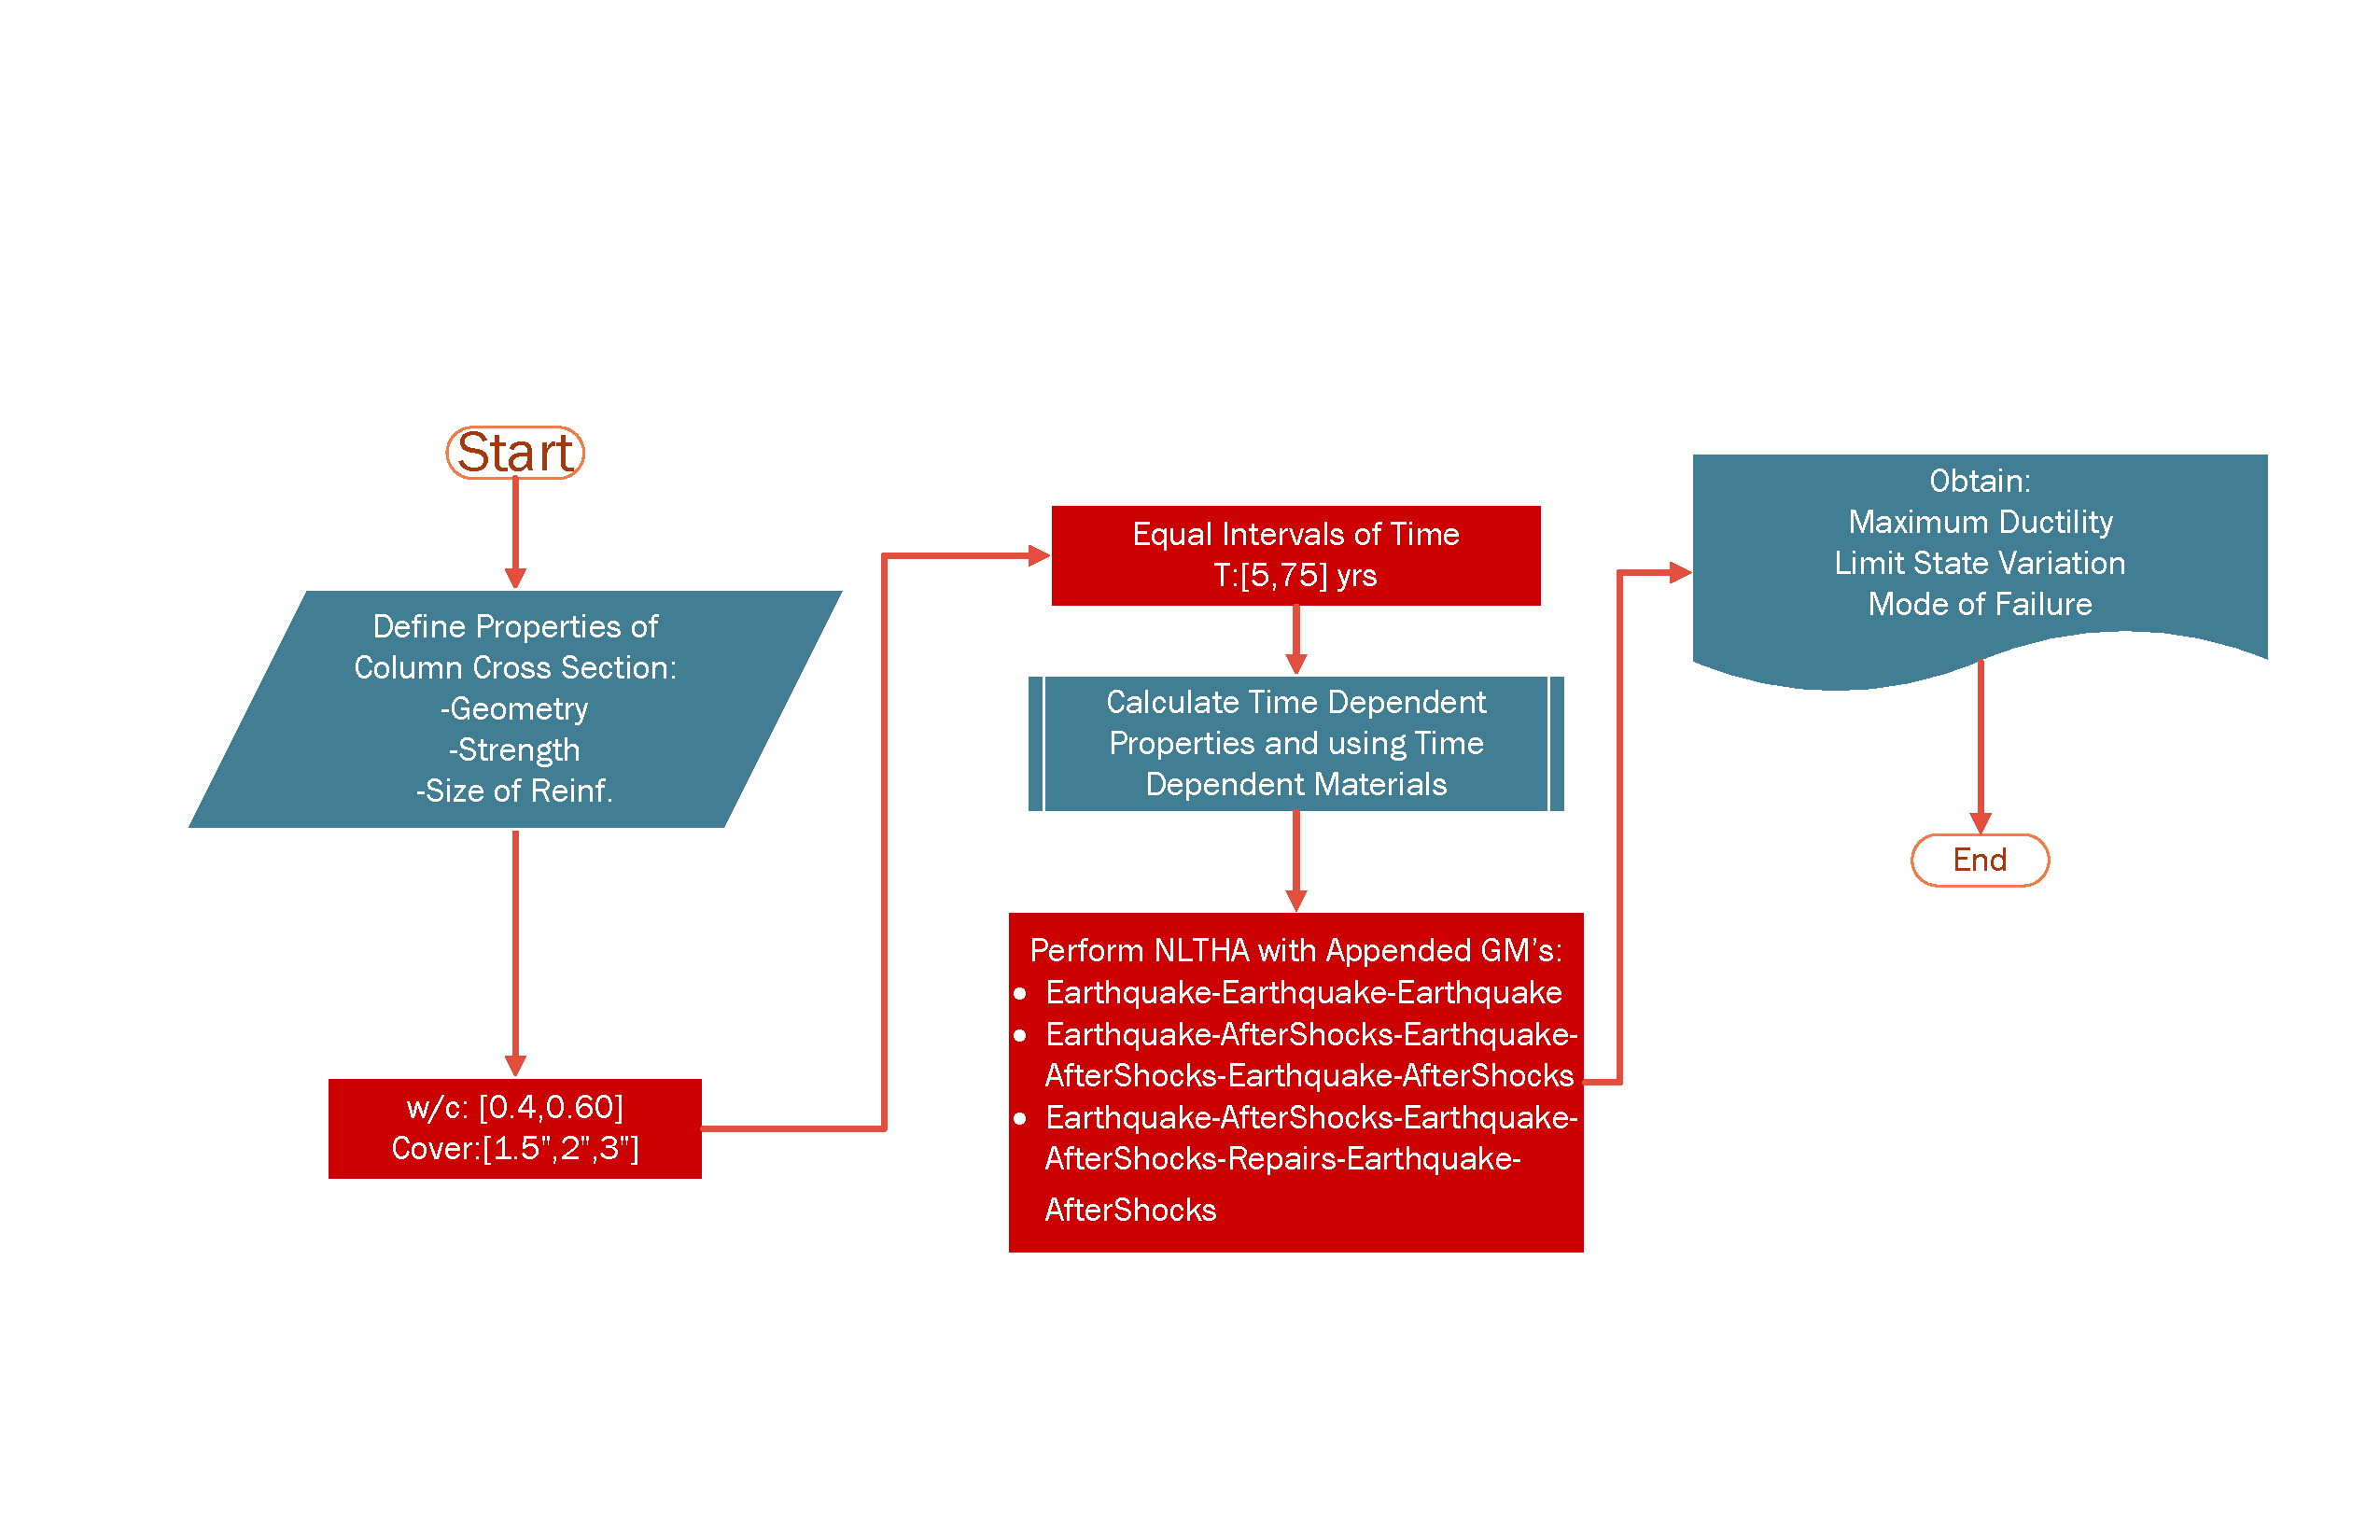
\includegraphics[width=0.9\textwidth]{Chapter-5/figs/AnalysisFramework_01}
	\caption{Analysis Framework Flowchart}
	\label{fig:NLTHA_Framework}
\end{figure}

\section{Earthquake selection}
\lipsum[4]
\section{Results from NLTHA}
\lipsum[5]
\subsection{Effect on structure response}
\lipsum[6]
\subsection{Effect on material response}
\lipsum[7]
\subsection{Preliminary results}
\lipsum[8]
